% This file was created by matlab2tikz.
%
%The latest updates can be retrieved from
%  http://www.mathworks.com/matlabcentral/fileexchange/22022-matlab2tikz-matlab2tikz
%where you can also make suggestions and rate matlab2tikz.
%
\definecolor{mycolor1}{rgb}{0.00000,0.44700,0.74100}%
%
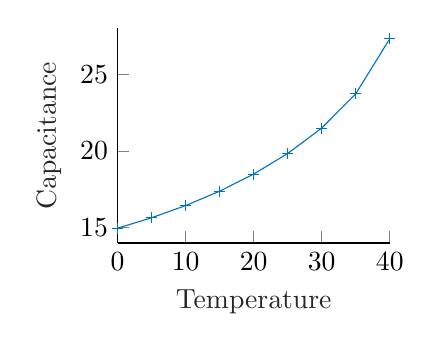
\begin{tikzpicture}

\begin{axis}[%
width=0.285\textwidth,
height=0.225\textwidth,
at={(0\textwidth,0\textwidth)},
scale only axis,
unbounded coords=jump,
xmin=0,
xmax=40,
xlabel style={font=\color{white!15!black}},
xlabel={Temperature \si{\celsius}},
ymin=14,
ymax=28,
ylabel style={font=\color{white!15!black}},
ylabel={Capacitance \si{\femto\farad}},
axis background/.style={fill=white},
axis x line*=bottom,
axis y line*=left
]
\addplot [color=mycolor1, mark=+, mark options={solid, mycolor1}, forget plot]
  table[row sep=crcr]{%
0	14.9688346633668\\
5	15.6501712728014\\
10	16.4436546810981\\
15	17.3805417263902\\
20	18.4961552351542\\
25	19.8364647423071\\
30	21.4934762266047\\
35	23.7269495667882\\
40	27.312717625232\\
45	nan\\
50	nan\\
55	nan\\
60	nan\\
65	nan\\
70	nan\\
75	nan\\
80	nan\\
85	nan\\
90	nan\\
95	nan\\
100	nan\\
};
\end{axis}
\end{tikzpicture}%